Ao logo dos últimos anos, o desafio proposto pelo projeto ImageNet  \emph{ImageNet Large Scale Visual Recognition Challenge} (ILSVRC) proporcionou o surgimento de algumas arquiteturas de CNNs que se tornaram bastante populares e são bastante utilizadas para resolver problemas dos mais diferentes domínios. As composições de algumas destas arquiteturas são detalhadas a seguir:

\paragraph{LeNet} Yann le Cun desenvolveu, em 1990, uma das primeiras arquiteturas utilizadas para o reconhecimento de dígitos manuscritos, a LeNet. Vencedora do ILSVRC 2010, esta arquitetura é composta por três camadas convolucionais alternadas com camadas de \textit{pooling} seguidas de duas FCLs conforme representado na Figura \ref{img:lenet} \cite{ref:sewak,ref:khan}.

\begin{figure}[!ht]
	\centering
	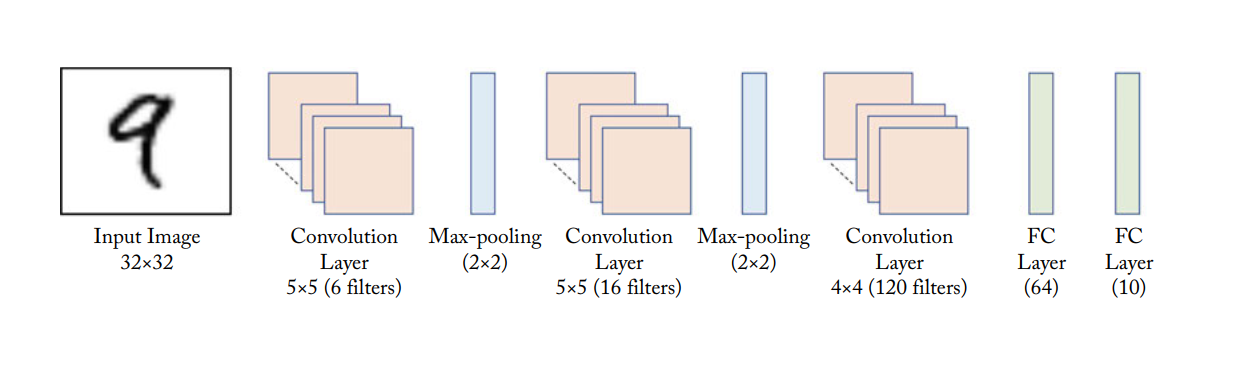
\includegraphics[width=1\textwidth]{./img/lenet}
	\caption{Representação da arquitetura de CNN LeNet. Fonte: \cite{ref:khan}.}
	\label{img:lenet}
\end{figure}


\paragraph{AlexNet} Em 2012 a vencedora do ILSVRC foi a arquitetura proposta por Alex Krizhevsky, conhecida como AlexNet. A AlexNet é mais profunda e uma versão muito mais ampla da arquitetura LeNet \cite{ref:satapathy}. A principal diferença entre a AlexNet e as CNNs predecessoras é a sua maior profundidade que lida muito bem com sua grande quantidade de parâmetros, além da utilização de artifícios como \textit{dropout} e \textit{data augmentation}. As cinco primeiras camadas da arquitetura AlexNet são camadas de convolução e \textit{pooling} alternadas de forma similar à LeNet, porém, seguem-se mais duas camadas uma convolucional e uma de\textit{pooling}. As três últimas camadas são FCL, mas além destas existem camadas \textit{dropout} que ajudam à reduzir \textit{overfiting}, o que resulta em uma melhor generalização \cite{ref:khan}. A AlexNet encontra-se representada na Figura \ref{img:alexnet}.

\begin{figure}[!ht]
	\centering
	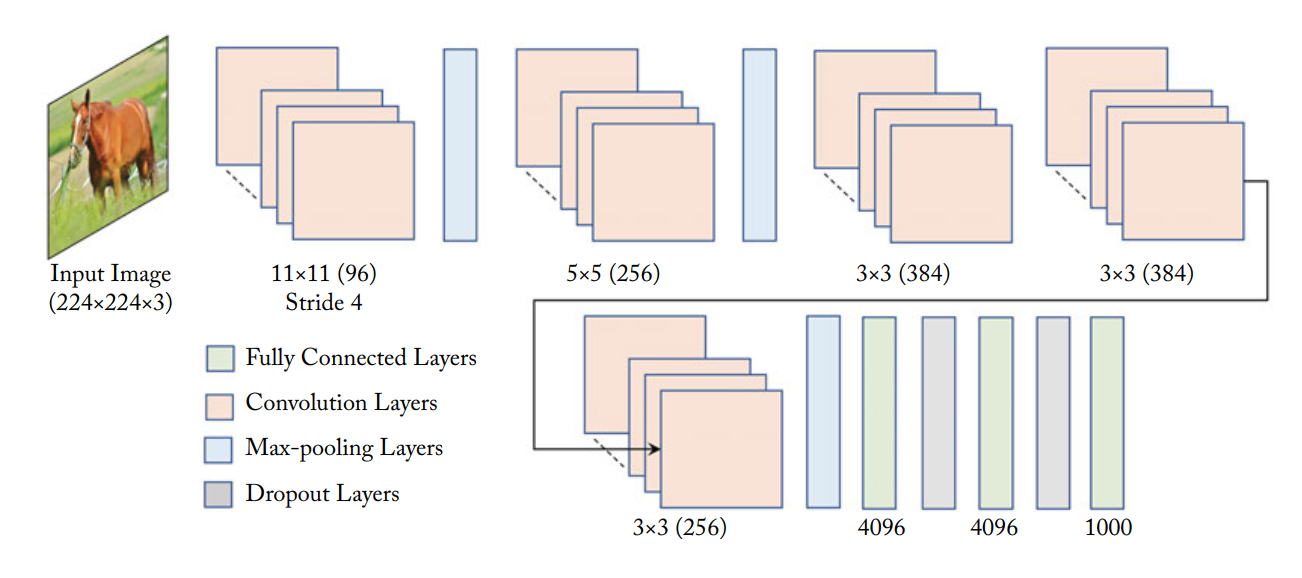
\includegraphics[width=1\textwidth]{./img/alexnet}
	\caption{Representação da arquitetura de CNN AlexNet. Fonte: \cite{ref:khan}.}
	\label{img:alexnet}
\end{figure}

\paragraph{VGGNet} A arquitetura VGGNet é uma das arquiteturas mais populares desde sua criação em 2014, apesar de não ter sido a vencedora do ILSVRC 2014. A razão de sua popularidade se dá pela simplicidade do modelo e pelo uso de pequenos ``\textit{kernels}'' de convolução que lidam muito bem com redes profundas por reduzirem o número de parâmetros o que aumenta a eficiência do treinamento. A arquitetura VGGNet usa estritamente \textit{kernels} de convolução de dimensão 3 x 3 combinados com camadas de \textit{pooling} para extração de características e um conjunto de três FCLs. Além das camadas de convolução, \textit{pooling} e das camadas conectadas, esta arquitetura também possui as camadas \textit{dropout} como pode ser observado na Figura \ref{img:vggnet} \cite{ref:khan}.

\begin{figure}[!ht]
	\centering
	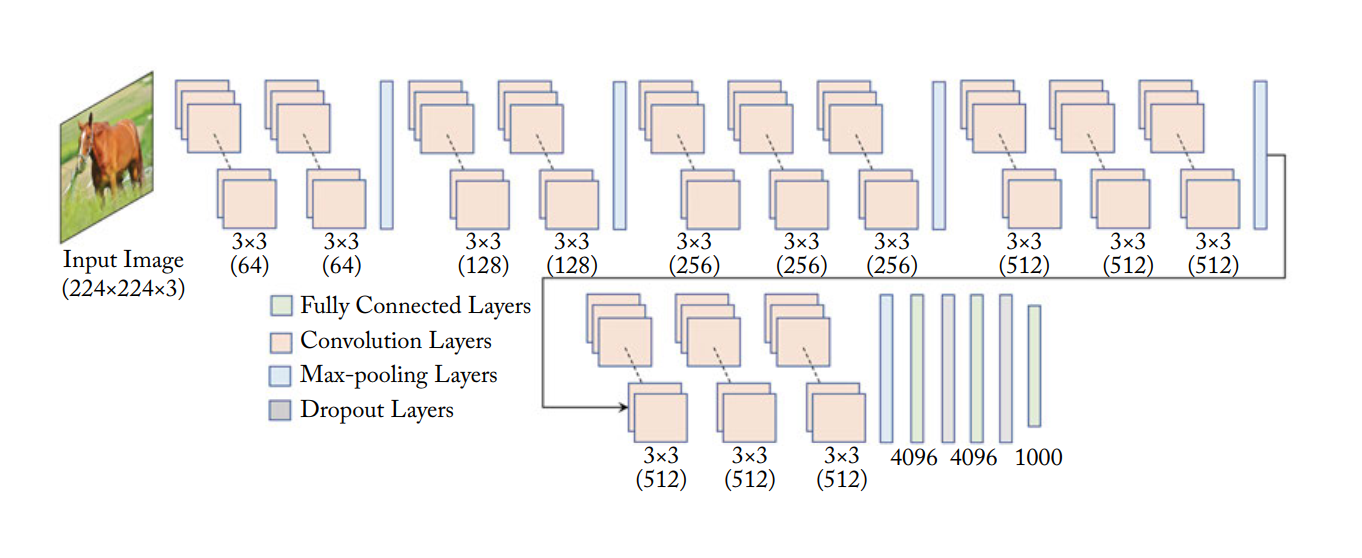
\includegraphics[width=1\textwidth]{./img/vggnet}
	\caption{Representação da arquitetura de CNN VGGNet. Fonte: \cite{ref:khan}.}
	\label{img:vggnet}
\end{figure}

\paragraph{GoogLeNet} Desenvolvida pela empresa Google e vencedora do ILSVRC 2014, a arquitetura GoogLeNet possui $22$ camadas baseadas em um módulo elementar chamado \emph{Inception Module}. O processamento desses módulos ocorre de forma paralela diferentemente do processamento sequencial das arquiteturas discutidas anteriormente. A ideia central da arquitetura GoogLeNet é paralelizar os módulos e combinar as características da saída sem se preocupar com as funções individuais de cada camada. No entanto, essa abordagem resulta em um mapa de características com muitos elementos, mas para contornar este problema, após a execução do primeiro módulo, a rede realiza uma redução de dimensionalidade utilizando uma FCL antes de continuar o processo de treinamento \cite{ref:khan}. A representação da arquitetura GoogLeNet encontra-se na Figura \ref{img:googlenet}.

\begin{figure}[!ht]
	\centering
	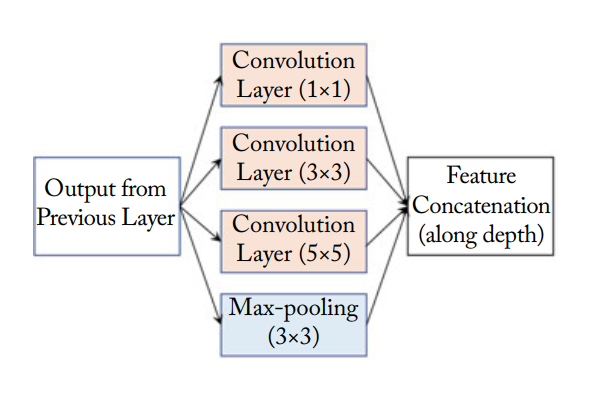
\includegraphics[width=0.6\textwidth]{./img/googlenet}
	\caption{Representação da arquitetura de CNN GoogLeNet. Fonte: \cite{ref:khan}.}
	\label{img:googlenet}
\end{figure}

